\section{Prototipos}
\label{seccion-prototipos}
A continuación se muestran los diferentes prototipos desarrollados durante la escritura de esta memoria. Los prototipos serán detallados utilizando una tabla resumen del mismo, la que incluye, los Objetivos del prototipo, una Descripción, los requisitos funcionales y no funcionales que aborda el prototipo.  Se incluyen las capturas del trabajo realizado, el análisis y conclusión del avance. Luego de la revisión de los prototipos, finalmente se detalla el desarrollo de las APIs, las cuales fueron desarrolladas en paralelo a los prototipos de la aplicación de configuración.

%En esta sección se muestran los prototipos desarrollados. Cada prototipo cuenta con una tabla para exponer el objetivo de éste, los requerimientos que aborda, imágenes del trabajo realizado y una conclusión sobre el avance del proyecto.

\subsection{Primer prototipo:  Activación de motores}
\label{primer-prototipo}
Este primer prototipo tiene como principal objetivo establecer las bases necesarias para conectar de OpenGlove con un dispositivo Android y establecer una comunicación básica. Para ello se utiliza la documentación oficial de Android sobre las conexiones bluetooth \footnote{Documentación oficial android: \url{https://developer.android.com/guide/topics/connectivity/bluetooth}}, permitiendo en primera instancia la obtención de dispositivos vinculados y la conexión con alguno de los mismos. No es necesaria la modificación de código cargado en la placa arduino, puesto que los protocolos de comunicación (mensajes) ya han sido establecidos con anterioridad. Por tanto se procede a hacer uso de la API en Java de bajo nivel desarrollada por Monsalve (2015). El prototipo se resume en la Tabla \ref{table:prototype-01}.

%\caption[Primer prototipo]{Primer prototipo \\ Fuente: elaboración propia (2018).}
%\label{table:prototype-01}

\begin{table}[H]
\caption[Primer prototipo: activación de motores]{Primer prototipo \\ Fuente: elaboración propia (2018).}
\label{table:prototype-01}
\begin{tabular}{|l|l|}
\hline
\textbf{ID del prototipo} & \textbf{P001}                                                                                                                                                                                                                                                                                                                                                                                                      \\ \hline
Nombre                    & Activación de motores                                                                                                                                                                                                                                                                                                                                                                                              \\ \hline
Objetivos                 & \begin{tabular}[c]{@{}l@{}}Verificar la correcta activación de motores en una aplicación \\ de Android nativo, utilizando las APIs de bajo nivel disponibles.\end{tabular}                                                                                                                                                                                                                                         \\ \hline
Descripción               & \begin{tabular}[c]{@{}l@{}}El primer prototipo desarrollado hace uso de la API de bajo nivel\\ de Java desarrollada por Monsalve (2015), sumándose modificaciones\\ realizadas para establecer la conexión en Android. Se obtiene\\ un prototipo capaz de establecer una conexión Bluetooth con\\ dispositivos previamente vinculados, permitiendo activar y \\ desactivar un motor de manera remota.\end{tabular} \\ \hline
Requisitos funcionales    & RF001                                                                                                                                                                                                                                                                                                                                                                                                             \\ \hline
Requisitos no funcionales & RNF002, RNF004                                                                                                                                                                                                                                                                                                                                                                                                     \\ \hline
\end{tabular}
\end{table}

\begin{figure}[H]
	\centering
	\captionsetup{justification=centering}
   	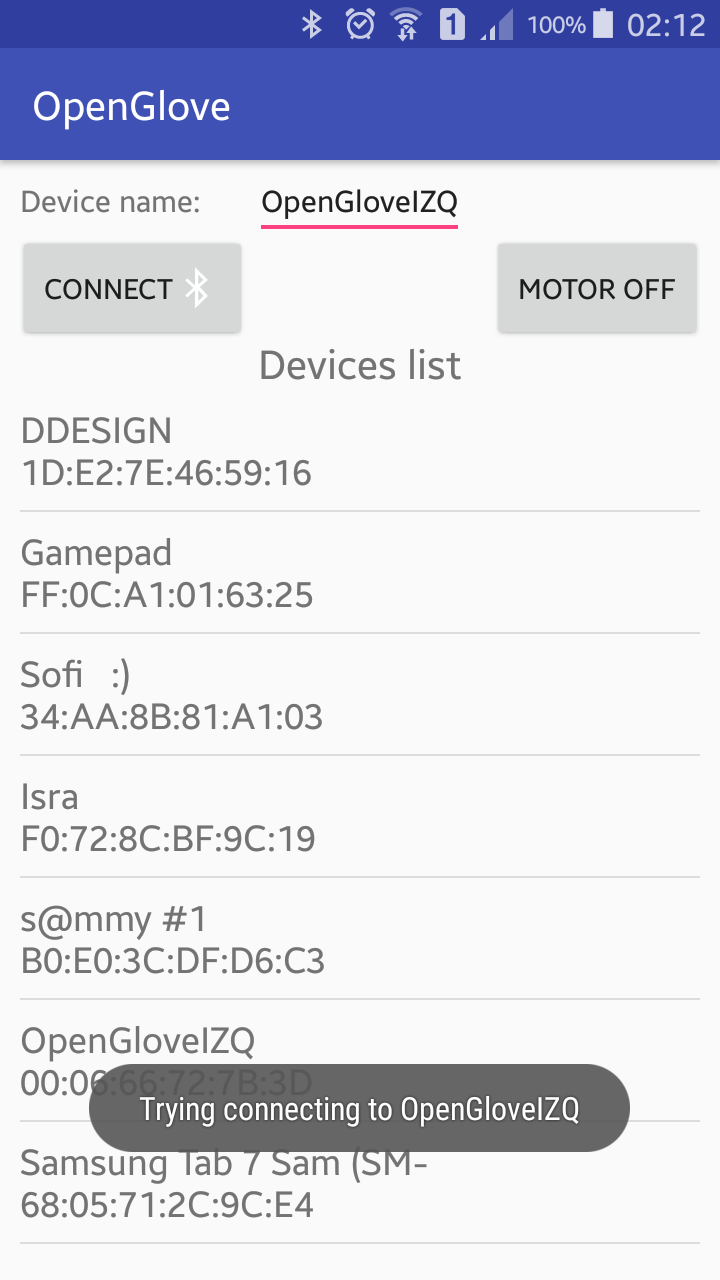
\includegraphics[width=0.3\textwidth]{images/chapter03/01-prototype.png} 
    \caption[Primer prototipo: activación de motores]{Primer prototipo: Activación de motores \\ Fuente: elaboración propia (2018).}
    \label{fig:prototype-01}
\end{figure}

Para lograr el objetivo propuesto, luego obtener los dispositivos vinculados y de la conexión con el guante mediante las APIs de bluetooth de Android, se procedió a enviar mensajes bajo el protocolo establecido en el desarrollo de Monsalve (2015). Dicho de una manera más detallada se utilizó la clase \textit{Message Generator} de la API de bajo nivel y la implementación nativa en Android para la escritura serial por medio de bluetooth. La Figura \ref{fig:prototype-01} consiste en el primer prototipo que muestra el listado de los dispositivos vinculados, la posibilidad de la conexión con el dispositivo deseado, permitiendo finalmente activar y desactivar el motor seleccionado para las pruebas. Para administrar la conexión entre los dispositivos, se requiere de un hilo\footnote{Hilo o Thread: En palabras muy resumidas, un hilo es una secuencia instrucciones dentro de un programa que se puede ejecutar independientemente de otro código, permitiendo así la ejecución en paralelo de instrucciones.} encargado de ello (\textit{ConnectedThread}), el cual se comunica con el hilo de la \textit{interfaz de usuario} (UI desde ahora)  mediante mensajes. El uso de hilos, permite administrar multiples conexiones con dispositivos Bluetooh de manera simultánea. En conclusión es posible realizar envio de mensajes bajo el protocolo que acepta OpenGlove desde una aplicación Android nativa en Java.



\subsection{Segundo prototipo: Obtención de datos desde los flexores}
\label{segundo-prototipo}
En el segundo prototipo se mantiene lo desarrollado previamente, añadiendo en esta iteración el soporte para los flexores. En este caso es necesaria la lectura desde el dispositivo OpenGlove. En la Tabla \ref{table:prototype-02} se muestra el resumen del prototipo ya mencionado. El RNF004 es cubierto parcialmente, debido a que se consulta continuamente el valor del flexor mediante funciones de bajo nivel, aumentando la latencia debido a las continuas consultas. No se presentan problemas de latencia para la activación y desactivación de motores.


%\caption[Segundo prototipo]{Segundo prototipo \\ Fuente: elaboración propia (2018).}
%\label{table:prototype-02}

\begin{table}[H]
\caption[Segundo prototipo: obtención de datos desde flexores]{Segundo prototipo\\ Fuente: elaboración propia (2018).}
\label{table:prototype-02}
\begin{tabular}{|l|l|}
\hline
\textbf{ID del prototipo} & \textbf{P002}                                                                                                                                                                                                                                                       \\ \hline
Nombre                    & Obtención de datos desde los flexores.                                                                                                                                                                                                                              \\ \hline
Objetivos                 & \begin{tabular}[c]{@{}l@{}}Verificar la correcta obtención de datos desde los flexores en \\ la aplicación de Android nativo, utilizando las APIs de bajo \\ nivel disponibles.\end{tabular}                                                                        \\ \hline
Descripción               & \begin{tabular}[c]{@{}l@{}}El segundo prototipo desarrollado agrega los métodos disponibles \\ de los flexores de la API de bajo nivel C\# hecha por Cerda (2017). \\ De esta manera, se obtiene un prototipo capaz de obtener los datos\\ del flexor.\end{tabular} \\ \hline
Requisitos funcionales    & RF001                                                                                                                                                                                                                                                              \\ \hline
Requisitos no funcionales & RNF002, RNF004 (parcialmente)
 \\ \hline
\end{tabular}
\end{table}


\begin{figure}[H]
	\centering
	\captionsetup{justification=centering}
   	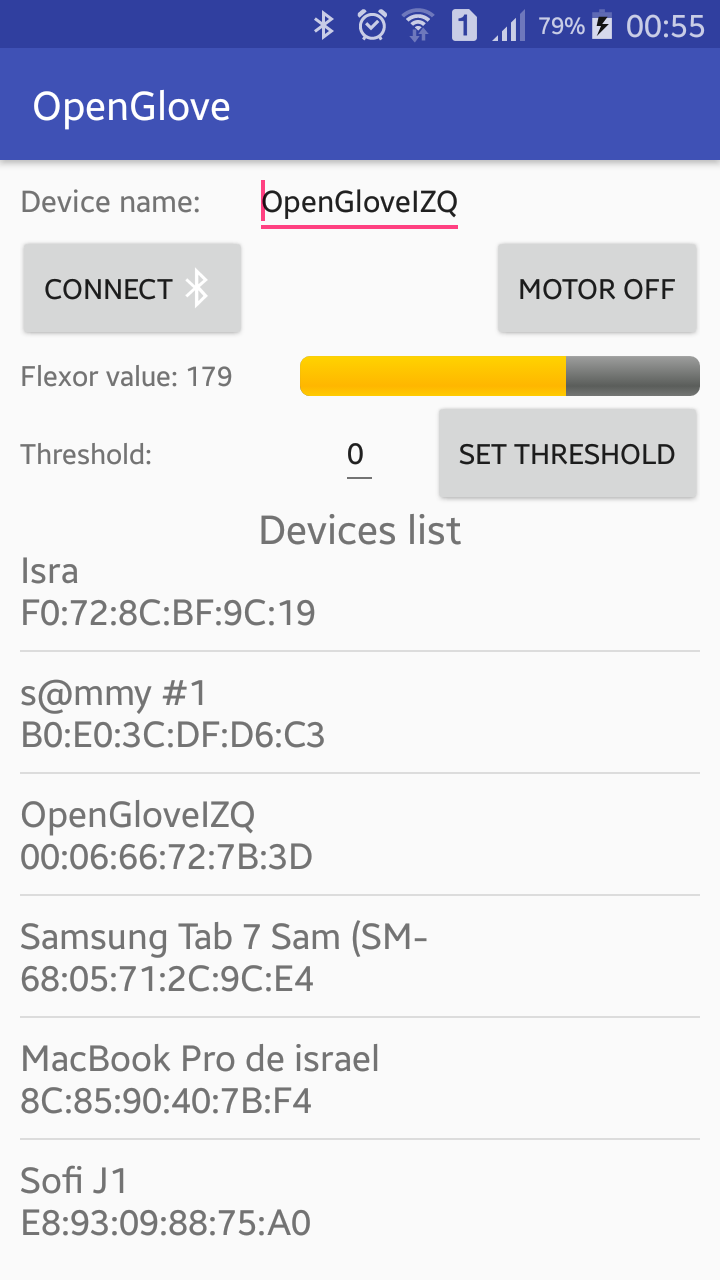
\includegraphics[width=0.3\textwidth]{images/chapter03/02-prototype.png} 
        \caption[Segundo prototipo: obtención de datos desde flexores]{Segundo prototipo: obtención de datos desde flexores \\ Fuente: elaboración propia (2018).}
    \label{fig:prototype-02}
\end{figure}

Para realizar la captura de datos del flexor, se obtiene valor actual del pin al cual el está conectado, esto se logra con el desarrollo de la función analogRead(pin) en Java basada en la API C\# de bajo nivel Cerda (2017). El hilo encargado de la administrar conexión (\textit{ConnectedThread}), tiene la responsabilidad de leer los mensajes desde OpenGlove y actualiza la UI enviando como un mensaje ente hilos el valor obtenido del flexor. Además se agregan las demás funciones de generación de mensajes relacionadas a los flexores en la API C\# ya mencionada. En la figura \ref{fig:prototype-02} se puede ver el estado actual del flexor el cual varia en un rango de entre 60 a 300 y 170 el valor medio del flexor sin aplicar fuerza.

\subsection{Tercer prototipo: Activación de motores y obtención de datos desde los flexores }
\label{tercer-prototipo}
% Xamarin C# prototype for cross platform use
En el segundo prototipo fue posible la activación del motor y obtener la información del flexor, permitiendo así comprobar la factibilidad de un desarrollo nativo en Android. En este tercer prototipo, se buscó dar soporte multiplataforma al proyecto, considerando la importancia de mantener umbrales de latencia, se optó por Xamarin. En concreto Xamarin.Forms,  que es una tecnología de desarrollo móvil multiplataforma \footnote{Traducción libre}, el cual permite desarrollar aplicaciones nativas para Android e iOS en C\#. La tabla \ref{table:prototype-03} muestra el resumen del tercer prototipo. El RNF004 es cubierto parcialmente, debido a que se consulta continuamente el valor del flexor al igual que el segundo prototipo. De igual manera no se presentan problemas de latencia para la activación y desactivación de motores.


%\caption[Tercer prototipo: activación de motores y obtención de datos desde flexores]{Tercer prototipo \\ Fuente: elaboración propia (2018).}
%\label{table:prototype-03}

\begin{table}[H]
\centering
\captionsetup{justification=centering}
\caption[Tercer prototipo: activación de motores y obtención de datos desde flexores]{Tercer prototipo \\ Fuente: elaboración propia (2018).}
\label{table:prototype-03}
\begin{tabular}{|l|l|}
\hline
\textbf{ID del prototipo} & \textbf{P003}                                                                                                                                                                                                                                                       \\ \hline
Nombre                    & Activación de motores y obtención de datos desde los flexores.                                                                                                                                                                                                                              \\ \hline
Objetivos                 & \begin{tabular}[c]{@{}l@{}}Verificar la correcta activación de motores y la obtención de \\ datos desde los flexores en la aplicación de Android nativo \\ con Xamarin.Forms, utilizando las APIs C\# de bajo nivel disponibles.\end{tabular}                                                                        \\ \hline
Descripción               & \begin{tabular}[c]{@{}l@{}}El tercer prototipo desarrollado agrega las mismas funcionalidades \\ que en el segundo prototipo.  De esta manera, se obtiene un prototipo \\ capaz de obtener los datos del flexor.\end{tabular} \\ \hline
Requisitos funcionales    & RF001                                                                                                                                                                                                                                                              \\ \hline
Requisitos no funcionales & RNF001, RNF002, RNF004 (parcialmente)                                                                                                                                                                                                                                                             \\ \hline
\end{tabular}
\end{table}



La figura \ref{fig:prototype-03} muestra el prototipo hecho en Xamarin.Forms, el cual es similar al segundo prototipo, con la diferencia en la forma de conectarse a un dispositivo bluetooth, el cual difiere en la forma de conectarse, este prototipo requiere presionar el dispositivo y aceptar el mensaje que explica el intento de conexión.


\begin{figure}[H]
	\centering
	\captionsetup{justification=centering}
   	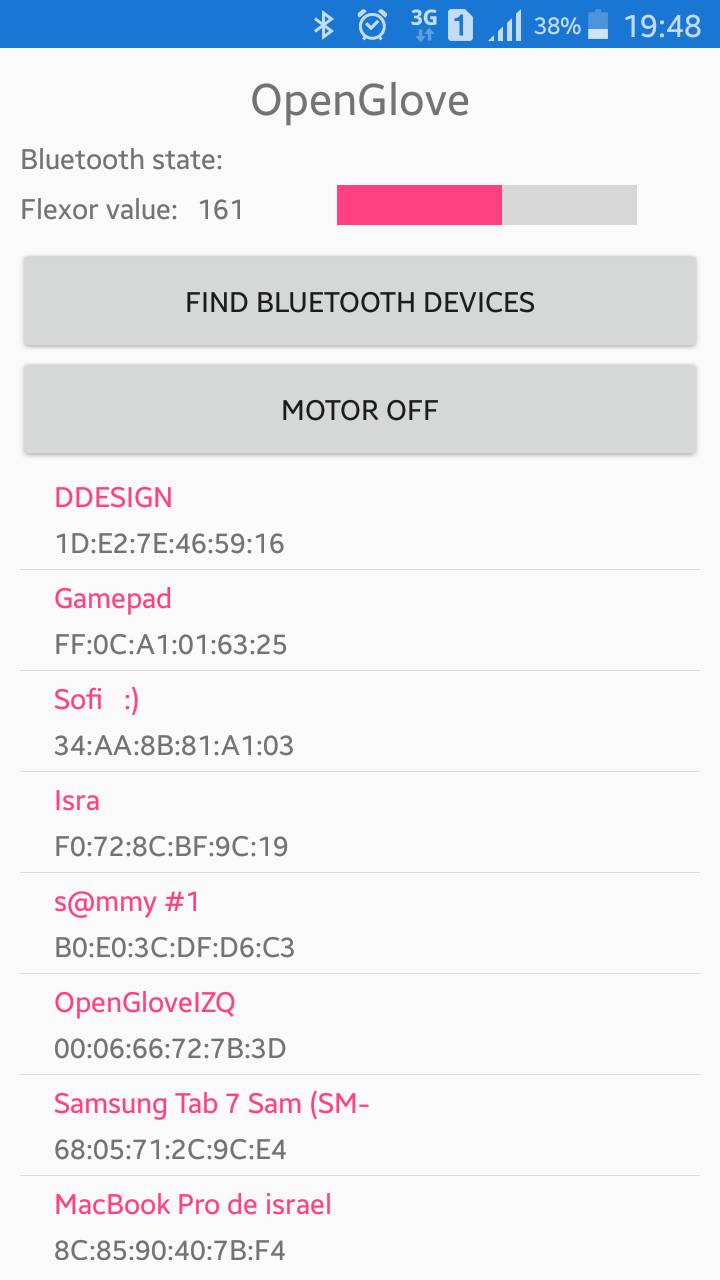
\includegraphics[width=0.3\textwidth]{images/chapter03/03-prototype.png} 
            \caption[Tercer prototipo: activación de motores y obtención de datos desde flexores]{Tercer prototipo: activación de motores y obtención de datos desde flexores \\ Fuente: elaboración propia (2018).}
    \label{fig:prototype-03}
\end{figure}





\subsection{Cuarto prototipo: Navegación aplicación, administración dispositivos Bluetooth, servidor WebSocket y configuración de la placa}
\label{cuarto-prototipo}
Este prototipo tiene como propósito cubrir los diferentes requisitos funcionales relacionados al comportamiento de la aplicación y ser la base de las siguientes iteraciones para dar soporte a los sensores de flexibilidad, actuadores e IMU. Se establece la navegación que posee la aplicación para hacer uso de todas las funcionalidades, por medio del diseño de un prototipo usando la herramienta AdobeXD en su versión grauita, con el cual se diseña, prototipa y se generan las diferentes imágenes e íconos que se utilizaron en el desarrollo del cuarto, quinto y sexto prototipo. La Figura \ref{fig:prototype-04}, muestra el prototipo desarrollado en Xamarin.Forms para Android y iOS, los cuales comparten la interfaz de usuario diferenciándose en la representaciones nativas de los elementos de cada plataforma. La Tabla \ref{table:prototype-04} muestra el resumen del prototipo ya mencionado.


%\caption[Cuarto prototipo]{Cuarto prototipo \\Fuente: elaboración propia (2018) }
%\label{table:prototype-04}

\begin{table}[H]
\caption[Cuarto prototipo]{Cuarto prototipo \\Fuente: elaboración propia (2018) }
\label{table:prototype-04}
\begin{tabular}{|l|l|}
\hline
\textbf{ID del prototipo} & \textbf{P004} \\ \hline
Nombre & \begin{tabular}[c]{@{}l@{}}Navegación aplicación, administración dispositivos Bluetooth, \\ servidor WebSocket y configuración de la placa.\end{tabular} \\ \hline
Objetivos & \begin{tabular}[c]{@{}l@{}}- Desarrollar Navegación de la aplicación (soporte iOS y Android).\\ - Desarrollar Administración de dispositivos Bluetooth.\\ - Desarrollar Administración del servidor WebSocket.\\ - Desarrollar la Configuración de la placa.\end{tabular} \\ \hline
Descripción & \begin{tabular}[c]{@{}l@{}}Este cuarto prototipo abarca los diferentes requisitos\\ funcionales relacionados al comportamiento de la aplicación y\\ de implementaciones de tecnología como el servidor WebSocket\\  embebido en la aplicación.\end{tabular} \\ \hline
Requisitos funcionales & RF001, RF002, RF003, RF004, RF008, RF010 \\ \hline
Requisitos no funcionales & RNF001, RNF002, RNF004 \\ \hline
\end{tabular}
\end{table}




\begin{figure}[H]
	\centering
	\captionsetup{justification=centering}
   	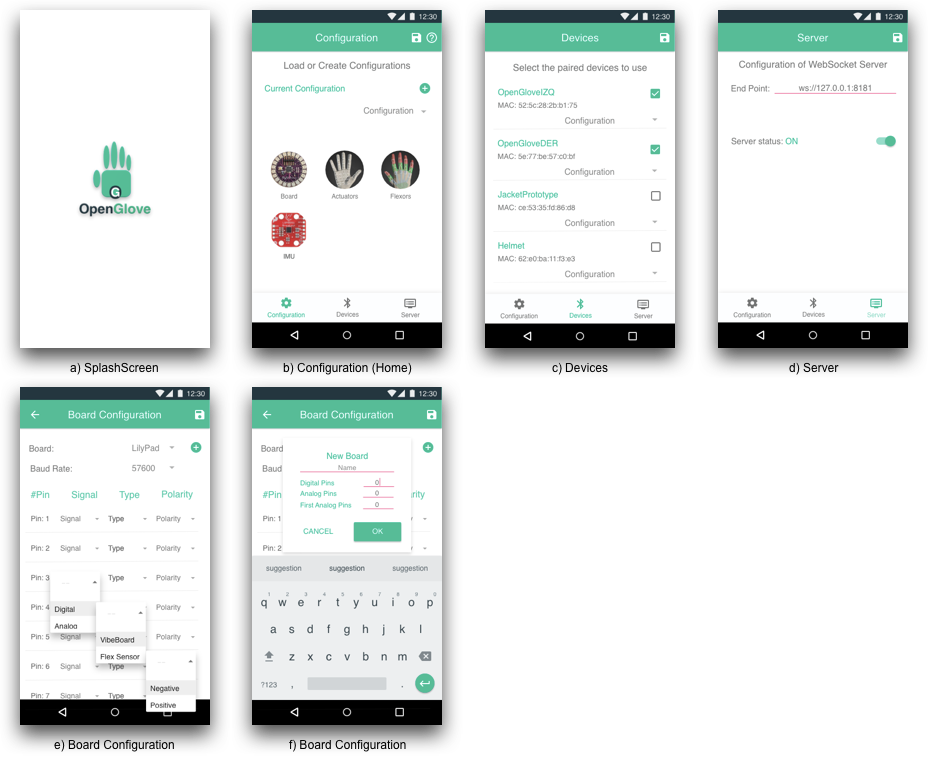
\includegraphics[width=1.0\textwidth]{images/chapter03/04-prototype/04-prototype.png} 
            \caption[Cuarto prototipo: app navigation, devices, server and board configuration]{Cuarto prototipo: app navigation, devices, server and board configuration \\ Fuente: elaboración propia (2018).}
    \label{fig:prototype-04}
\end{figure}

A continuación se describen las pantallas desarrolladas, especificando el alcance de las mismas para iOS y Android.

\begin{itemize}

\item La Figura \ref{fig:prototype-04}.a muestra el SplashScreen de la aplicación, el cual se muestra mientras se inicia la aplicación. \textbf{[Soporte completo: iOS y Android]}

\item La Figura \ref{fig:prototype-04}.b muestra el menú principal de la aplicación de configuración, en el cual es posible cargar configuraciones existentes o bien crear una nueva configuración, la cual contiene la configuración de la placa, de los actuadores, de los flexores y del sensor IMU. Esta aplicación seleccionada o creada puede ser modificada del menú principal accediendo a las pantallas que permiten configurar la placa, actuadores, flexores e IMU. La aplicación posee una navegación basada en BottomNavigation, la cual corresponde a una	 barra de navegación inferior que permite acceder al menú de configuración general, la configuración de dispositivos Bluetooth y la configuración del servidor. \textbf{[Soporte completo: iOS y Android]}

\item La Figura \ref{fig:prototype-04}.c muestra una lista con los dispositivos Bluetooth emparejados, permitiendo ver el nombre y dirección MAC de ellos. También permite elegir los dispositivos Bluetooth que se utilizarán junto la configuración que se le desee aplicar. La aplicación en iOS no puede mostrar la lista de dispositivos emparejados, no se implementó la clase Communication para el proyecto iOS, porque está fuera del alcance de este trabajo \textbf{[Soporte completo: Android]}.

\item La Figura \ref{fig:prototype-04}.d muestra la pantalla referente al servidor WebSocket, permitiendo definir la dirección de acceso al servidor y el encendido y apagado del mismo. Para la implementación del servidor WebSocket se utilizó el paquete de software Fleck, el que se encuentra disponible en la plataforma NuGet \footnote{Paquetes de software NuGet https://www.nuget.org/packages} junto a otros paquetes que pueden ser utilizados si son compatibles con la versión .NET standar 2.0. Con este paquete se desarrolló la clase OpenGloveServer para su uso en la aplicación de configuración. En esa clase se instancia un servidor y  donde se establecen los EventHandler necesarios para mandar mensajes entre los hilos que administran las conexiones de sus dispositivos Bluetooth (clase Communication) y el servidor WebSocket (clase OpenGloveServer) \textbf{[Soporte completo: iOS y Android]}.

\item La Figura \ref{fig:prototype-04}.e muestra la pantalla que permite definir la configuración de la placa, creando una nueva placa o utilizando alguna previamente creada, como puede ser la placa LilyPad utilizada en este trabajo. En esta pantalla de la aplicación, se puede elegir o crear una placa y seleccionar el BaudRate \footnote{El baud rate especifica la velocidad en la que se envían los datos por una línea serial, usualmente son expresadas en unidades de bits por segundo (bps). \url{https://learn.sparkfun.com/tutorials/serial-communication/rules-of-serial}
} con el que se trabajará. Luego de ello se procede a configurar los pines de placa considerando la configuración física de los mismos, definiendo el tipo de señal, pines digitales y análogos, si el pin corresponde a flexor o un actuador e indicando su polaridad, positiva o negativa \textbf{[Soporte completo: iOS y Android]}.

\item La Figura \ref{fig:prototype-04}.f muestra el diálogo utilizado para crear una nueva configuración de placa, pidiendo el nombre de la placa, el pin donde comienzan los pines análogos (depende de la placa específica \citep{tesis-cerda-rodrigo}), cantidad de pines digitales y análogos \textbf{[Soporte completo: iOS y Android]}.

\end{itemize}






\subsection{Quinto  prototipo: Mapeo de actuadores y prueba de actuadores}
\label{quinto-prototipo}
Este prototipo tiene como propósito cubrir los diferentes requisitos funcionales relacionados a los actuadores.  La Tabla \ref{table:prototype-05} muestra el resumen del prototipo antes mencionado. Este prototipo utilizó como base el cuarto prototipo desarrollado.

%\caption[Quinto prototipo]{Quinto prototipo \\Fuente: elaboración propia (2018)}
%\label{table:prototype-05}

\begin{table}[H]
\caption[Quinto prototipo]{Quinto prototipo \\Fuente: elaboración propia (2018)}
\label{table:prototype-05}
\begin{tabular}{|l|l|}
\hline
\textbf{ID del prototipo} & \textbf{P005}                                                                                                                                                                                     \\ \hline
Nombre                    & Mapeo de actuadores y prueba de actuadores                                                                                                                                                        \\ \hline
Objetivos                 & \begin{tabular}[c]{@{}l@{}}- Desarrollar el mapeo actuador-region\\ - Desarrollar la prueba de actuadores\end{tabular}                                                                            \\ \hline
Descripción               & \begin{tabular}[c]{@{}l@{}}Este quinto prototipo abarca los diferentes requisitos\\ funcionales relacionados a los actuadores, sumándose\\ a lo desarrollado en el cuarto prototipo.\end{tabular} \\ \hline
Requisitos funcionales    & \begin{tabular}[c]{@{}l@{}}RF001, RF002, RF003, RF004, RF005, RF006, RF007,\\ RF008, RF009, RF010, RF011\end{tabular}                                                                             \\ \hline
Requisitos no funcionales & RNF001, RNF002, RNF004                                                                                                                                                                            \\ \hline
\end{tabular}
\end{table}

\begin{figure}[H]
	\centering
	\captionsetup{justification=centering}
   	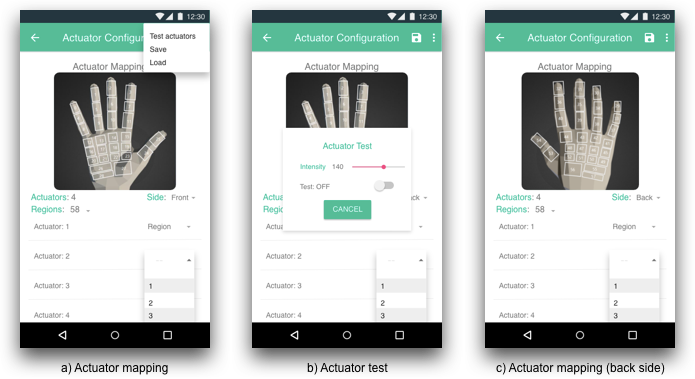
\includegraphics[width=1.0\textwidth]{images/chapter03/05-prototype/05-prototype.png} 
            \caption[Quinto prototipo: actuator mapping and  actuator test]{Quinto prototipo: actuator mapping and actuator test \\ Fuente: elaboración propia (2018).}
    \label{fig:prototype-05}
\end{figure}

En paralelo al desarrollo de este prototipo fue necesario el desarrollo de la API C\#, es decir el desarrollo de un cliente WebSocket utilizando el paquete de software WebSocketSharp\footnote{WebSocketSharp: \url{https://www.nuget.org/packages/WebSocketSharp/1.0.3-rc11}}. El cliente es quien envía mensajes al servidor que está dentro de la aplicación de configuración, para activar los actuadores deseados. Para ello se incluyen métodos para la activación de motores, en el cual se especifica el dispositivo Bluetooth y una lista de regiones a activar, las cuales son traducidas a los mensajes generados por la API de bajo nivel de OpenGlove.

A continuación se describen las pantallas desarrolladas, especificando el alcance de las mismas para iOS y Android.

\begin{itemize}

\item La Figura \ref{fig:prototype-05}.a muestra la pantalla que permite el mapeo actuador-región, mostrando una lista de los actuadores identificados desde la configuración de la placa. Es posible cambiar la imagen que representa el mapeo del dispositivo Bluetooth, para ello se requiere definir la cantidad de regiones que posee el lado frontal y trasero al momento de definir la cantidad de regiones, especificando también el número inicial que identifica a las regiones (iniciando en 1 o en 0 por ejemplo). El mapeo se realiza seleccionando la región desde una lista desplegable en cada actuador, la cual es generada dependiendo de la configuración inicial de la cantidad de regiones. \textbf{[Soporte completo: iOS y Android]}.

\item La Figura \ref{fig:prototype-05}.b muestra el diálogo que permite realizar las pruebas de los actuadores mapeados, permitiendo iniciar y detener la prueba con la intensidad seleccionada. La prueba se termina una vez se cierra el diálogo o se desactiva dentro del diálogo. La aplicación en iOS no puede activar regiones mapeadas, porque no se implementó la clase Communication para el proyecto iOS, porque está fuera del alcance de este trabajo \textbf{[Soporte completo: Android]}.

\item La Figura \ref{fig:prototype-05}.c muestra el segundo lado de la imagen de mapeo de actuadores, de la pantalla de mapeo mostrada en la Figura \ref{fig:prototype-05}.a.

\end{itemize}




\subsection{Sexto  prototipo: Mapeo de flexores, prueba de flexores y la configuración del IMU.}
\label{sexto-prototipo}
Este prototipo tiene como propósito cubrir los diferentes requisitos funcionales relacionados a los flexores e IMU. Se utilizó como base el quinto prototipo ya descrito. 

Este prototipo tiene como propósito cubrir los diferentes requisitos funcionales relacionados a los flexores e IMU.  La Tabla \ref{table:prototype-06} muestra el resumen del prototipo antes mencionado. Este prototipo utilizó como base el quinto prototipo desarrollado.

%\caption[Sexto prototipo]{Sexto prototipo \\Fuente: elaboración propia (2018)}
%\label{table:prototype-06}

\begin{table}[H]
\caption[Sexto prototipo]{Sexto prototipo \\Fuente: elaboración propia (2018)}
\label{table:prototype-06}
\begin{tabular}{|l|l|}
\hline
\textbf{ID del prototipo} & \textbf{P006}                                                                                                                                                                                                                                                                                                             \\ \hline
Nombre                    & \begin{tabular}[c]{@{}l@{}}Mapeo de flexores, prueba de flexores y la configuración\\ del IMU.\end{tabular}                                                                                                                                                                                                               \\ \hline
Objetivos                 & \begin{tabular}[c]{@{}l@{}}- Desarrollar el mapeo flexor-region\\ - Desarrollar la prueba de flexores\\ - Desarrollar la configuración del IMU\end{tabular}                                                                                                                                                               \\ \hline
Descripción               & \begin{tabular}[c]{@{}l@{}}Este sexto prototipo abarca los diferentes requisitos\\ funcionales relacionados a los flexores e IMU, sumándose\\ a lo desarrollado en el quinto prototipo. Esto es posible\\ gracias al desarrollo de la API C\#, la cual es replicada para\\ el lenguaje de programación Java.\end{tabular} \\ \hline
Requisitos funcionales    & \begin{tabular}[c]{@{}l@{}}RF001, RF002, RF003, RF004, RF005, RF006, RF007,\\ RF008, RF009, RF010, RF011, RF012, RF013, RF014,\\ RF015, RF016, RF018, RF019, RF020, RF021, RF022,\\ RF023\end{tabular}                                                                                                                    \\ \hline
Requisitos no funcionales & RNF001, RNF002, RNF003, RNF004, RNF005, RNF006                                                                                                                                                                                                                                                                            \\ \hline
\end{tabular}
\end{table}


\begin{figure}[H]
	\centering
	\captionsetup{justification=centering}
   	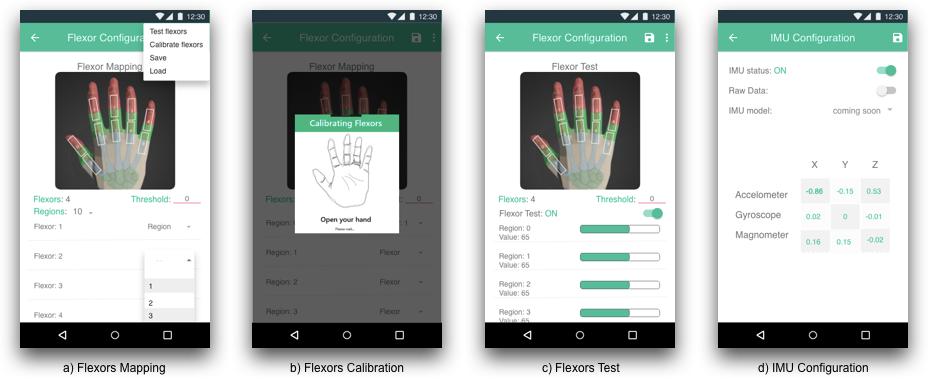
\includegraphics[width=1.0\textwidth]{images/chapter03/06-prototype/06-prototype.png} 
            \caption[Sexto prototipo: flexor mapping, flexor test and IMU configuration]{Sexto prototipo: flexor mapping, flexor test and IMU configuration\\ Fuente: elaboración propia (2018).}
    \label{fig:prototype-06}
\end{figure}

De igual manera al quinto prototipo, se agregan métodos que permiten el desarrollar las funcionalidades referentes a los flexores e IMU, permitiendo definir el Threshold (límite en que, se enviará un dato de un flexor si la diferencia es mayor o igual a este valor), agregar o remover flexores de una región, calibrar los flexores y confirmar la calibración. También permite iniciar o detener el IMU y definir si recibir datos crudos o procesados.

A continuación se describen las pantallas desarrolladas, especificando el alcance de las mismas para iOS y Android.

\begin{itemize}

\item La Figura \ref{fig:prototype-06}.a muestra la pantalla de mapeo flexor-region de igual manera que el de actuadores, agregando la asignación del Threshold que se utilizará cuando en la prueba de flexores y cuando se le asigne la configuración al o los dispositivos Bluetooth. \textbf{[Soporte completo: iOS y Android]}.

\item La Figura \ref{fig:prototype-06}.b muestra una pantalla sobrepuesta con una animación, la cual indica que es necesario mover las articulaciones para calibrar los flexores. La aplicación en iOS no puede calibrar los flexores, porque no se implementó la clase Communication para el proyecto iOS, porque está fuera del alcance de este trabajo \textbf{[Soporte completo: Android]}.

\item La Figura \ref{fig:prototype-06}.c muestra la pantalla que permite probar los flexores previamente mapeados, también se puede definir el Threshold antes de activar o desactivar la prueba de los flexores. La aplicación en iOS no puede obtener datos de los flexores, porque no se implementó la clase Communication para el proyecto iOS, porque está fuera del alcance de este trabajo \textbf{[Soporte completo: Android]}.

\item La Figura \ref{fig:prototype-06}.d muestra la pantalla de configuración del sensor de rastreo IMU, en la cual se puede iniciar o detener el mismo, configurar el envío de datos crudos o procesados. También permite ver los datos recibidos por el acelerómetro, giroscopio y magnetómetro para los ejes $X$, $Y$ y $Z$.Agregar soporte a otros modelos de sensores de rastreo IMU. No es posible seleccionar otro modelo de IMU aparte de SparkFun LSM9DS1, dado que requiere bibliotecas de software específicas en el código de la placa Arduino. Podría definirse que la selección de modelo de placa IMU, permita cargar código en la placa Arduino, incluyendo a las librerías y código específico del modelo del IMU. Esto podría ser realizado utilizando la conexión Bluetooth o por medio de conexión USB adecuada. Por ejemplo, la herramienta Bluino Loader - Arduino IDE\footnote{Bluino Loader: https://www.hackster.io/mansurkamsur/upload-sketch-arduino-over-bluetooth-using-android-f1ce55} permite cargar código a la placa Arduino por Bluetooth o USB. La aplicación en iOS no puede calibrar obtener datos desde el IMU, porque no se implementó la clase Communication para el proyecto iOS, porque está fuera del alcance de este trabajo \textbf{[Soporte completo: Android]}.

\end{itemize}
